The decay \btodsphi proceeds via the annihilation of the \Bp mesons constituent quarks into
a virtual \Wp boson in the SM\footnote{
  This analysis was published in \Ref{LHCb-PAPER-2012-025}.}.
To achieve the final state, the \Wp decays into a $\cquark\squarkbar$ pair and an additional
$\squark\squarkbar$ pair must be \emph{popped} from the QCD field.
This is the only diagram that can perpetuate such a decay at tree level because the initial state
quarks are all different to those in the final state.
Annihilation decays of \Bp mesons are rare in the SM due to the magnitude of $|\V{ub}|$ (see
\Eq{eq:th:vub}); in fact, no fully hadronic decays proceeding via annihilation have yet been
observed.


Predictions for the brancing fraction $\BF\big(\btodsphi\big)$ are calculated using the OPE defined
by the effective Hamiltonian~\cite{Zou:2009zza,Mohanta:2002wf,PhysRevD.76.057701,Lu:2001yz}:
\begin{equation}
  \Ham{eff}=
  -4\frac{G_F}{\sqrt{2}} \V{ub}\Vconj{cs}
  \big[
    C_1(\Lambda)\Op{1}+C_2(\Lambda)\Op{2}
    \big]
\end{equation}
where
\begin{align}
  \Op{1} &= \big(\bquarkbar\gamma_\mu P_Lu\big) \big(\cquarkbar\gamma_\mu P_Ls\big) \nonumber\\
  \Op{2} &= \big(\bquarkbar\gamma_\mu P_Ls\big) \big(\cquarkbar\gamma_\mu P_Lu\big).
\end{align}
and $C_{1,2}$ are Wilson coefficients defined at scale $\Lambda=m_b$.
Projection operators $P_{L,R}$ are defined as $P_L=\tfrac12(1-\gamma_5)$ and
$P_R=\tfrac12(1+\gamma_5)$.
The short distance operators \Op{1} and \Op{2} both describe the transition $b\!\to scu$.
Despite the relatively simple effective Hamiltonian, QCD effects make $\BF\big(\btodsphi\big)$ very
difficult to predict.
Figure~\ref{fig:dsphi:feyn} shows hows Feynman diagrams for a first order decay of \btodsphi in the
SM and SUSY, where the \ssbar pair are produced by a decaying gluon which could have
originated from any of the four quarks.
If the gluon were to be from one of the initial state quarks then the assumption of factorization
does not hold.


\begin{figure}
  \begin{center}
    %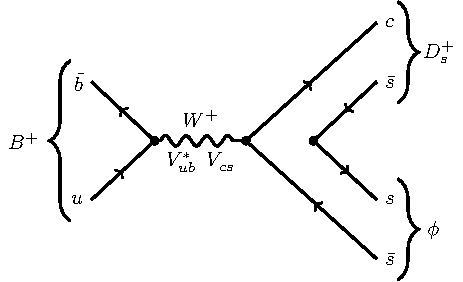
\includegraphics[width=0.48\textwidth]{feynman_dsphi_sm}
    %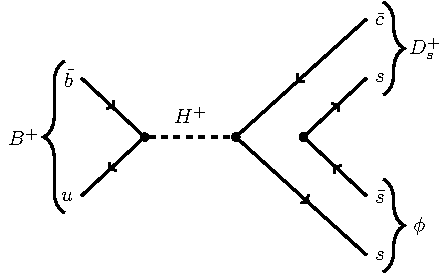
\includegraphics[width=0.48\textwidth]{feynman_dsphi_susy}
    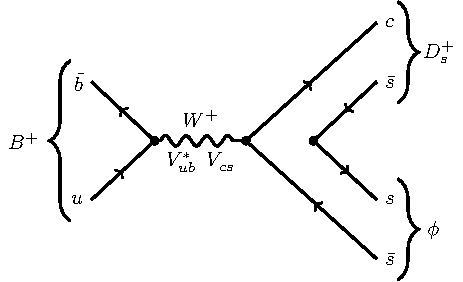
\includegraphics[scale=1]{feynman_dsphi_sm}
    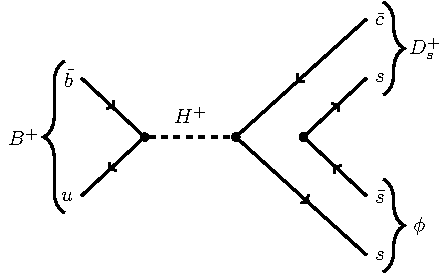
\includegraphics[scale=1]{feynman_dsphi_susy}
    \caption[Feynman diagram for the decay \btodsphi]
    {\small
      A Feynman diagram for the decay \btodsphi being mediated by a
      (left) \Wp in the SM, and
      (right) $H^+$ in SUSY.
      The diagrams shown here are the colour favoured diagrams, the \ssbar from the gluon can form
      a \phii meson, but this is colour suppressed.
    }
    \label{fig:dsphi:feyn}
  \end{center}
\end{figure}


Predictions for the branching fraction $\BF(\btodsphi)$ in the SM are in
the range (1--7)$\e{-7}$~\cite{Zou:2009zza,Mohanta:2002wf,PhysRevD.76.057701,Lu:2001yz}.
The large range in branching fraction predictions is due to the difficulties in modelling the
hadronization of the final state quarks; the hadronic form-factors lead to large uncertainties.
Calculating the decay dynamics is further complicated because the decay \btodsphi is not fully
factorizable, since the \ssbar pair can come from the final state quarks (factorizable) or the
initial quarks, in which case they contribute to the short range process.

Significant enhancements in $\BF\big(\btodsphi\big)$
could be observed were the decay to be mediated by additional BSM
particles.
Figure~\ref{fig:dsphi:feyn} shows Feynman diagrams for a first order decay of \btodsphi in the SM
and SUSY.
Reference~\cite{Mohanta:2002wf} makes prediccctions for the branching fraction of the decay
\btodsphi in the \sm, as well as in a model with two Higgs-doublets (2HDM) and an $R$-parity
violating model (RPV):
\begin{align}
  %\BF\big(\btodsphi\big)_\mathrm{SM}&=0.67\e{-6}, \nonumber\\
  %\BF\big(\btodsphi\big)_\mathrm{2HDM}&=\pz8.0\e{-6}, \nonumber\\
  %\BF\big(\btodsphi\big)_\mathrm{RPV}&=3.06\e{-4}.
  \BF\big(\btodsphi\big)|{\makebox[\widthof{$_\mathrm{2HDM}$}][l]{$_\mathrm{SM}$}}
  &=0.67\e{-6}, \nonumber\\
  \BF\big(\btodsphi\big)|_\mathrm{2HDM}
  &=8.0\pz\e{-6}, \nonumber\\
  \BF\big(\btodsphi\big)|{\makebox[\widthof{$_\mathrm{2HDM}$}][l]{$_\mathrm{RPV}$}}
  &=3.06\e{-4}.
\end{align}
These numbers indicate that, while the exact \sm value of $\BF\big(\btodsphi\big)$ is not well
known, the value for models with additional mediating particles could be enhanced significnaly.


The \CP asymmetry, \acp, of the decay could also indicate \np.
In the SM $\acp=0$, because the Feynman diagram only contains one phase (in \V{ub}), but
interference from BSM physics diagrams can alter this significantly.
Predictions from \Ref{Mohanta:2002wf} are:
\begin{align}
  \acp\big(\btodsphi\big)|_\mathrm{2HDM}
  &\leq 59\,\%, \nonumber\\
  \acp\big(\btodsphi\big)|{\makebox[\widthof{$_\mathrm{2HDM}$}][l]{$_\mathrm{RPV}$}}
  &\leq 14\,\%.
\end{align}
So, both measurements of $\BF\big(\btodsphi\big)$ and $\BF\big(\btodsphi\big)$ could lead to
evidence of \np particles.

Further motivation for studying the decay \btodsphi comes from the
historical conflict between the measurements of \V{ub} from inclusive semi-leptonic decays and
from the decay $\decay{\Bp}{\taup\nu_\tau}$, see \Sec{sec:bsm:faisec:bsm:fail}.
The schematic Feynman diagram for \btodsphi is identical to $\decay{\Bp}{\taup\nu_\tau}$
--- except that an \ssbar pair must be produced in the case of the former.
Since the publication of this analysis, \Ref{Crivellin:2014zpa} has concluded that the
discrepancies cannot explained by new physics, and rather is due to underestimated uncertainties in
either theory or experiment.

%In addition to searching for the decay \btodsphi it is a trivial extension to also look for the
%decay \bctodsphi, which is also an annihilation type decay and has the same schematic Feynman
%diagram.
%This will be much more suppressed due to the difference in production cross-section of the \Bp and
%\Bc mesons.

%The analysis was done on $1\invfb$ of data collected by the \lhcb detector in 2011 from $pp$
%collisions with a centre-of-mass energy of $7\tev$.




%Previous experimental limit by \babar \cite{Aubert:2005gd}
%\begin{equation}
  %\BF\big(\btodsphi\big) < 1.8\e{-6} \qquad \text{90\,\% C.L.}
%\end{equation}



\subsection{Other annihilation-type hadronic decays}
The annihilation of the \Bp meson can perpetuate numerous decays resulting in fully hadronic
states, including a charmed meson.
The decay \decay{\Bp}{\Dp\Kstarz} proceeds in the same way as
\btodsphi, but the former needs a \ddbar pair to be created from the QCD field rather than an
\ssbar pair.
Similarly, the decay \decay{\Bp}{\Ds\Kstarzb} is identical to the \btodsphi excepting that instead
of \decay{\Wp}{\cquark\squarkbar} the \Wp decays into an $\cquark\dquarkbar$ pair.
In addition, it is trivial to search for the heavily suppressed decays
\decay{\Bp}{\Dp\Kstarzb} and \decay{\Bp}{\Ds\Kstarz}.
All these decay transitions can propagate from a decaying \Bc meson.

While the decays mentioned in the above paragraph are not covered in this thesis, limits for each
were set in \Ref{LHCb-PAPER-2012-025}.






























